

%----------------------------------------------------------------------------------------
%	PACKAGES AND OTHER DOCUMENT CONFIGURATIONS
%----------------------------------------------------------------------------------------

\documentclass[a0,portrait]{a0poster}

\usepackage{multicol} % This is so we can have multiple columns of text side-by-side
\columnsep=50pt % This is the amount of white space between the columns in the poster
\columnseprule=0pt % This is the thickness of the black line between the columns in the poster

\usepackage[svgnames]{xcolor} % Specify colors by their 'svgnames', for a full list of all colors available see here: http://www.latextemplates.com/svgnames-colors

\usepackage{times} % Use the times font
%\usepackage{palatino} % Uncomment to use the Palatino font

\graphicspath{{figures/}} % Location of the graphics files
\usepackage{booktabs} % Top and bottom rules for table
\usepackage[font=small,labelfont=bf]{caption} % Required for specifying captions to tables and figures
\usepackage{amsfonts, amsmath, amsthm, amssymb} % For math fonts, symbols and environments
\usepackage{wrapfig} % Allows wrapping text around tables and figures
% \usepackage[labelformat=empty]{caption}
\usepackage{fontawesome}
\usepackage[utf8]{inputenc}

\begin{document}

%----------------------------------------------------------------------------------------
%	POSTER HEADER 
%----------------------------------------------------------------------------------------

% The header is divided into two boxes:
% The first is 75% wide and houses the title, subtitle, names, university/organization and contact information
% The second is 25% wide and houses a logo for your university/organization or a photo of you
% The widths of these boxes can be easily edited to accommodate your content as you see fit

\begin{minipage}[b]{0.75\linewidth}
\VeryHuge \color{NavyBlue} \textbf{Evaluating dengue forecasting models to 
predict Zika and Chikungunya in Brazil.}
\color{Black}\\[0.4cm] 
\Large \textbf{
\authorName{Flávio Codeço Coelho}{1\space\Letter}, 
\authorName{Elisa Mussumeci}{1}, 
%\authorName{N.~Gustafsson}{1}, 
\authorName{Marcelo Orgler}{1}, 
\authorName{Linneu Holanda}{1}} 
% Author(s)
\\
\vspace{1cm}
\large \textbf{
\authorAffil{1}{Fundação Getulio Vargas, Brazil}; 
\large \textbf{Correspondence to: fccoelho@fgv.br}}
\begin{center}
    \large \textbf{Poster DOI: ADD here from figshare \\ \faGithub \ 
github.com/AlertaDengue | \faTwitter \ @fccoelho}
\end{center}
\end{minipage}
%
\begin{minipage}[b]{0.25\linewidth}
\begin{center}

\includegraphics[width=15cm]{figures/Marca_FGV_EMAp.png}\\ 

\includegraphics[width=16cm]{figures/geomed.png}\\
\end{center}
\end{minipage}

%\vspace{.2cm} % A bit of extra whitespace between the header and poster content

%----------------------------------------------------------------------------------------

\begin{multicols}{3} % This is how many columns your poster will be broken into, a portrait poster is generally split into 2 columns

%----------------------------------------------------------------------------------------
%	ABSTRACT
%----------------------------------------------------------------------------------------

\noindent
The Mosquito Aedes aegypti is a vector for multiple viruses around the globe. Its distribution is restricted to tropical and subtropical climates, which reflects its sensitivity to temperature, humidity and other weather constraints. The modulation of its life cicle by climate, shapes the seasonality of the diseases it transmits.
 In Brazil, Aedes aegypti has been mainly associated with the transmission of 
dengue, making it a marked seasonal disease. In recent years, A. aegypti has 
also been notably responsible for epidemics of the Zika and Chikungunya virus. 
In this paper we explore the performance of dengue forecast models trained on 
the longer available incidence timeseries to predict the weekly incidence of 
Zika and Chikungunya as well.  We will use a LSTM (long short term memory) 
recursive neural network model, which we have shown, in a previous work, to 
yield accurate forecasts for weekly dengue incidence. We will also compare it 
to a Random Quantile Forest model. Climate variables such as temperature, 
humidity, and atmospheric pressure are also used as predictors. A spatial 
component built from the incidence at neighboring cities is also included. We 
present results of the forecast of total incidence of arboviral disease as well 
as of each disease separately and discuss the relative performances of the model 
for each of these tasks.

\begin{center}\vspace{1cm}
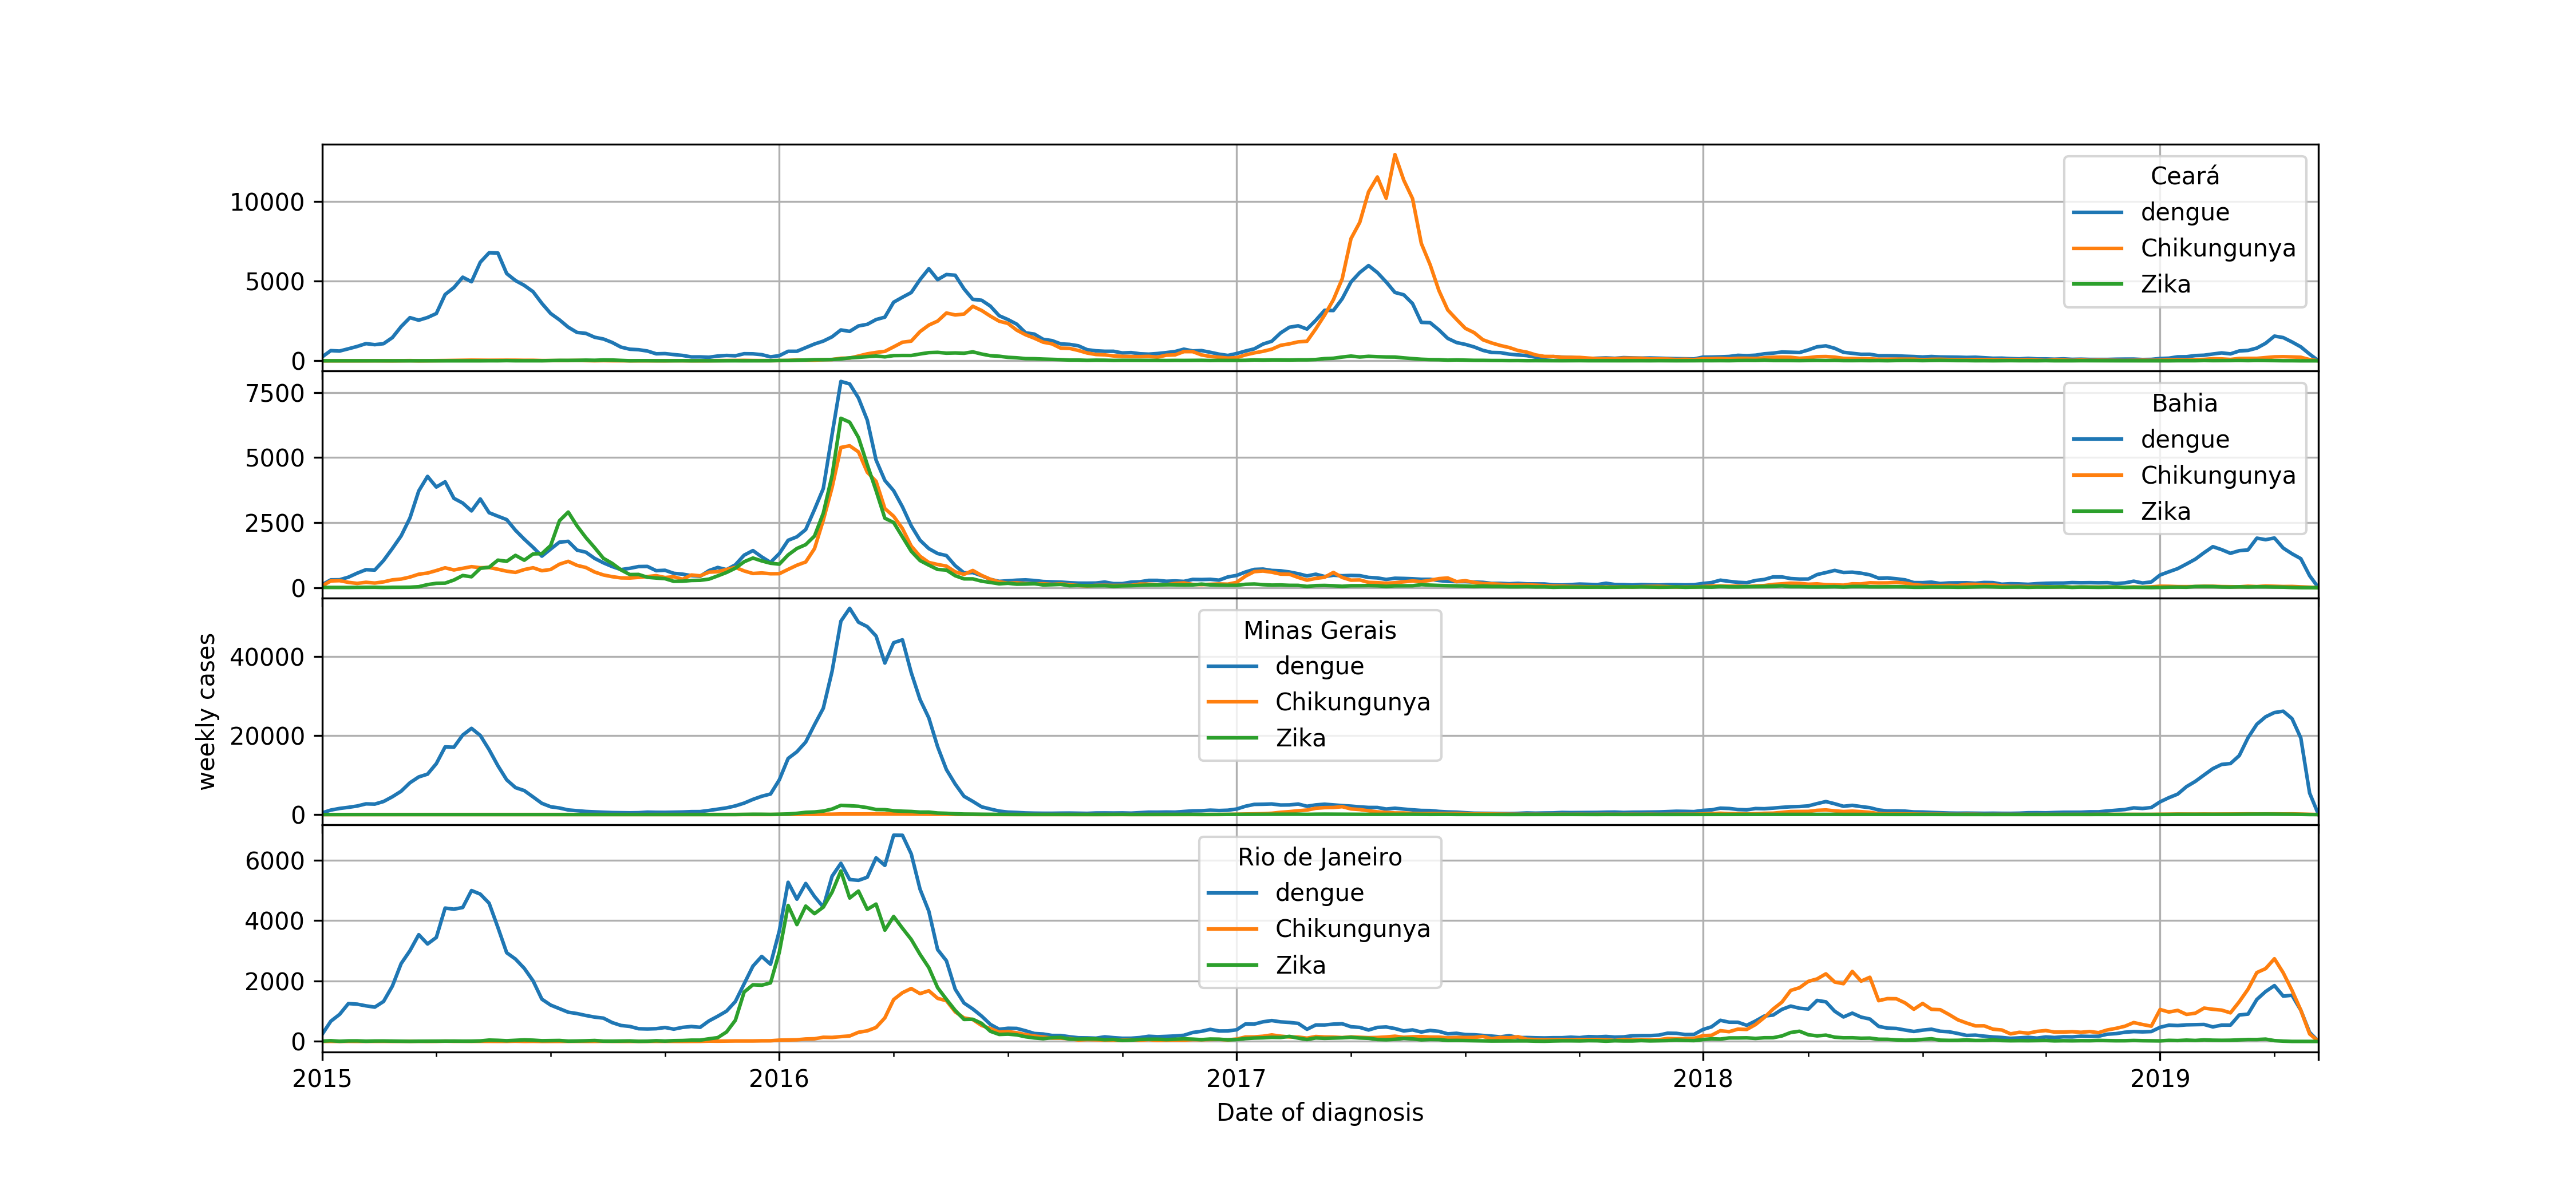
\includegraphics[width=\linewidth]{figures/dcz_series.png}
\captionof{figure}{\textbf{Weekly incidence for the state of Ceará, Brazil.} 
The three arboviroses incidences are correlated.}
\label{fig:series}
\end{center}%\vspace{1cm}

The data used in this work comes from the Infodengue project, which monitors 
these arboviroses in Brazil. In the figure \ref{fig:series} we can see the 
incidence series for states in Brazil which had significant outbreaks of the 3 
arboviroses since 2016 when Chikungunya and Zika arrived in Brazil.
%----------------------------------------------------------------------------------------
%	NanoJ-Core: Drift Correction
%----------------------------------------------------------------------------------------
\section*{Three diseases, one vector.}

\noindent
Given their similar transmission mechanisms, these diseases present similar 
seasonal patterns. Being seasonal diseases with serious consequences, being 
able to forecast their incidence is very important for public health 
authorities. Among these, Dengue is the one with the longest historic records. 
Therefore its worth investigating how usefull our knowledge about dengue 
dynamics is to predict other arboviroses, in this case Zika and Chikungunya. 
Here we will revisit a forecast model developed by the authors for dengue, and 
evaluate its performance in predicting the other two arboviroses.




%----------------------------------------------------------------------------------------
%	NanoJ-Core: Channel registration
%----------------------------------------------------------------------------------------
\section*{Dengue forecast models}
\subsection*{LSTM}
\noindent
A LSTM model is a recurrent deep neural network model developed to handle 
predictions of timeseries. We used a LSTM model with 3 LSTM units followed by 
3 dropout layers. The model was trained for 300 epochs using a mean-log 
squared-error (MLSE) loss function  and a Nesterov Adam 
optimizer\cite{sutskever2013importance}. A look back of 4 weeks and a 
forecasting window of 4 weeks were used.

\begin{center}\vspace{1cm} 
    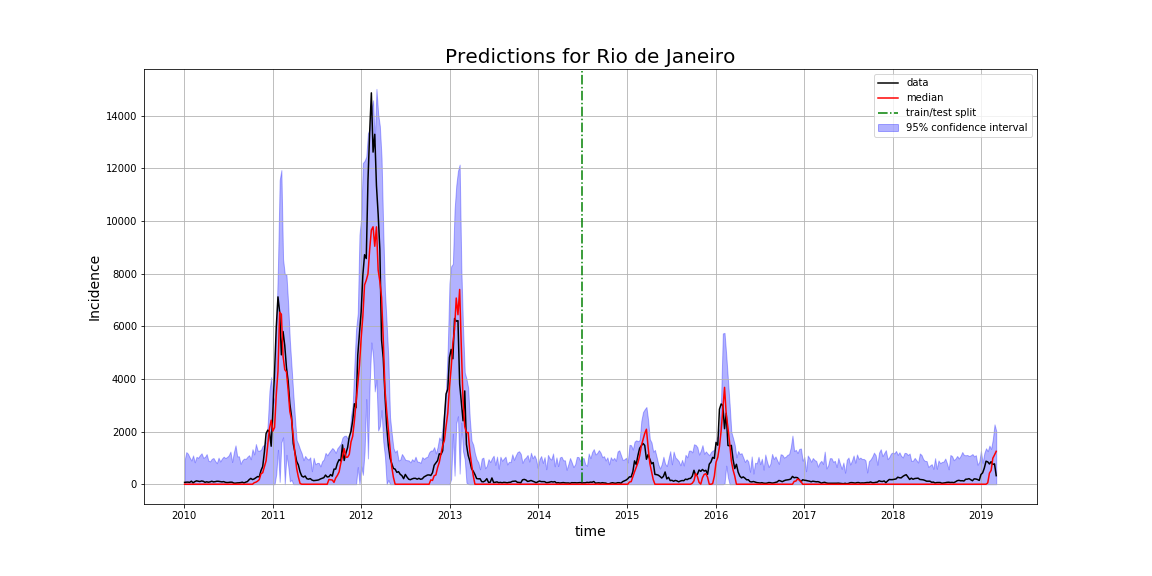
\includegraphics[width=\linewidth]{figures/LSTM_dropout.png}
    \captionof{figure}{\textbf{LSTM forecast for Dengue incidence (black line)} 
Prediction (red line) with 95\% interval for dengue.}
\end{center}%\vspace{1cm}

\subsection*{Random Quantile Forest (RQF)}
Random Forest models calculate an ensemble of regression trees from random 
subsets of data. RQF model are an extension to regular random forests in which 
the full conditional distribution of $Y$ given $X=x$ is calculated. As a 
result, it is a non-parametric, consistent and accurate way to determine 
conditional quantiles from high-dimensional 
predictors\cite{meinshausen2006quantile}.
\section*{Results}

\noindent
Both models were fitted to available Chickungunya and Zika data yielding...

\begin{center}\vspace{1cm}
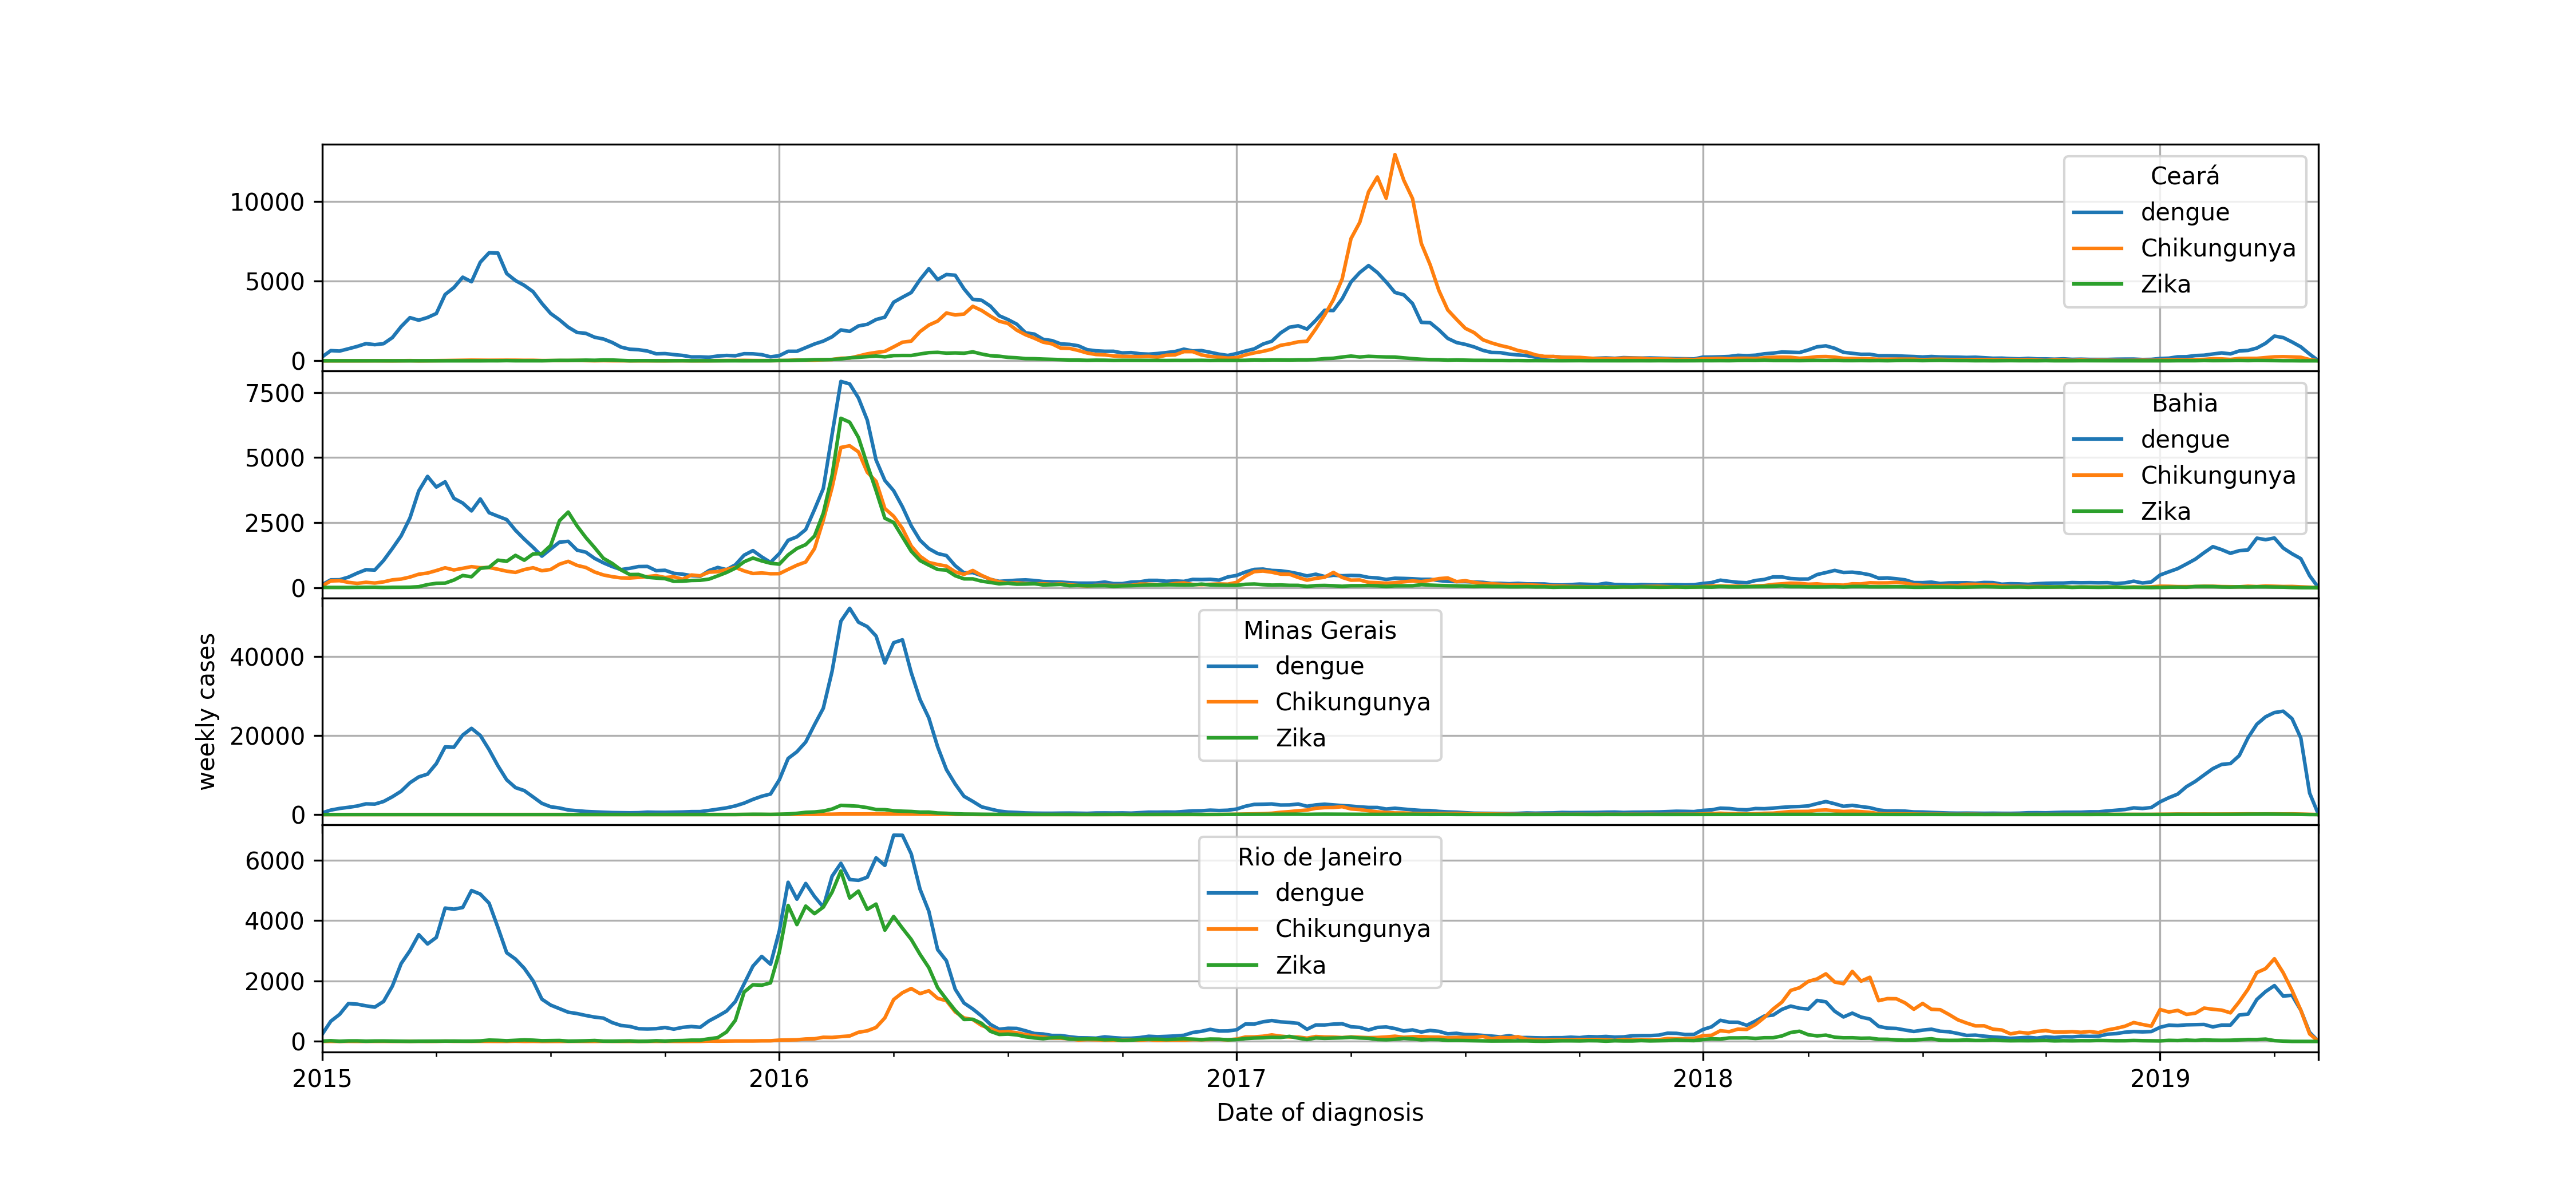
\includegraphics[width=\linewidth]{figures/dcz_series.png}
\captionof{figure}{\textbf{Live-cell super-resolution microscopy with NanoJ-SRRF.} \textbf{a)} Comparison of widefield and SRRF reconstruction from UtrCH-GFP actin labelling. Scale bar: 5 \textmu{}m. \textbf{b)} Time-course of the inset shown in a), obtained at 33.3 Hz and displayed every 30 s. Scale bar: 1 \textmu{}m. \textbf{c)} Colour-coded time course. Scale bar: 1 \textmu{}m.}
\end{center}%\vspace{1cm}

%----------------------------------------------------------------------------------------
%	NanoJ-SQUIRREL: Estimating Image Quality & Resolution
%----------------------------------------------------------------------------------------
\section*{Discussion}


\begin{center}\vspace{1cm}
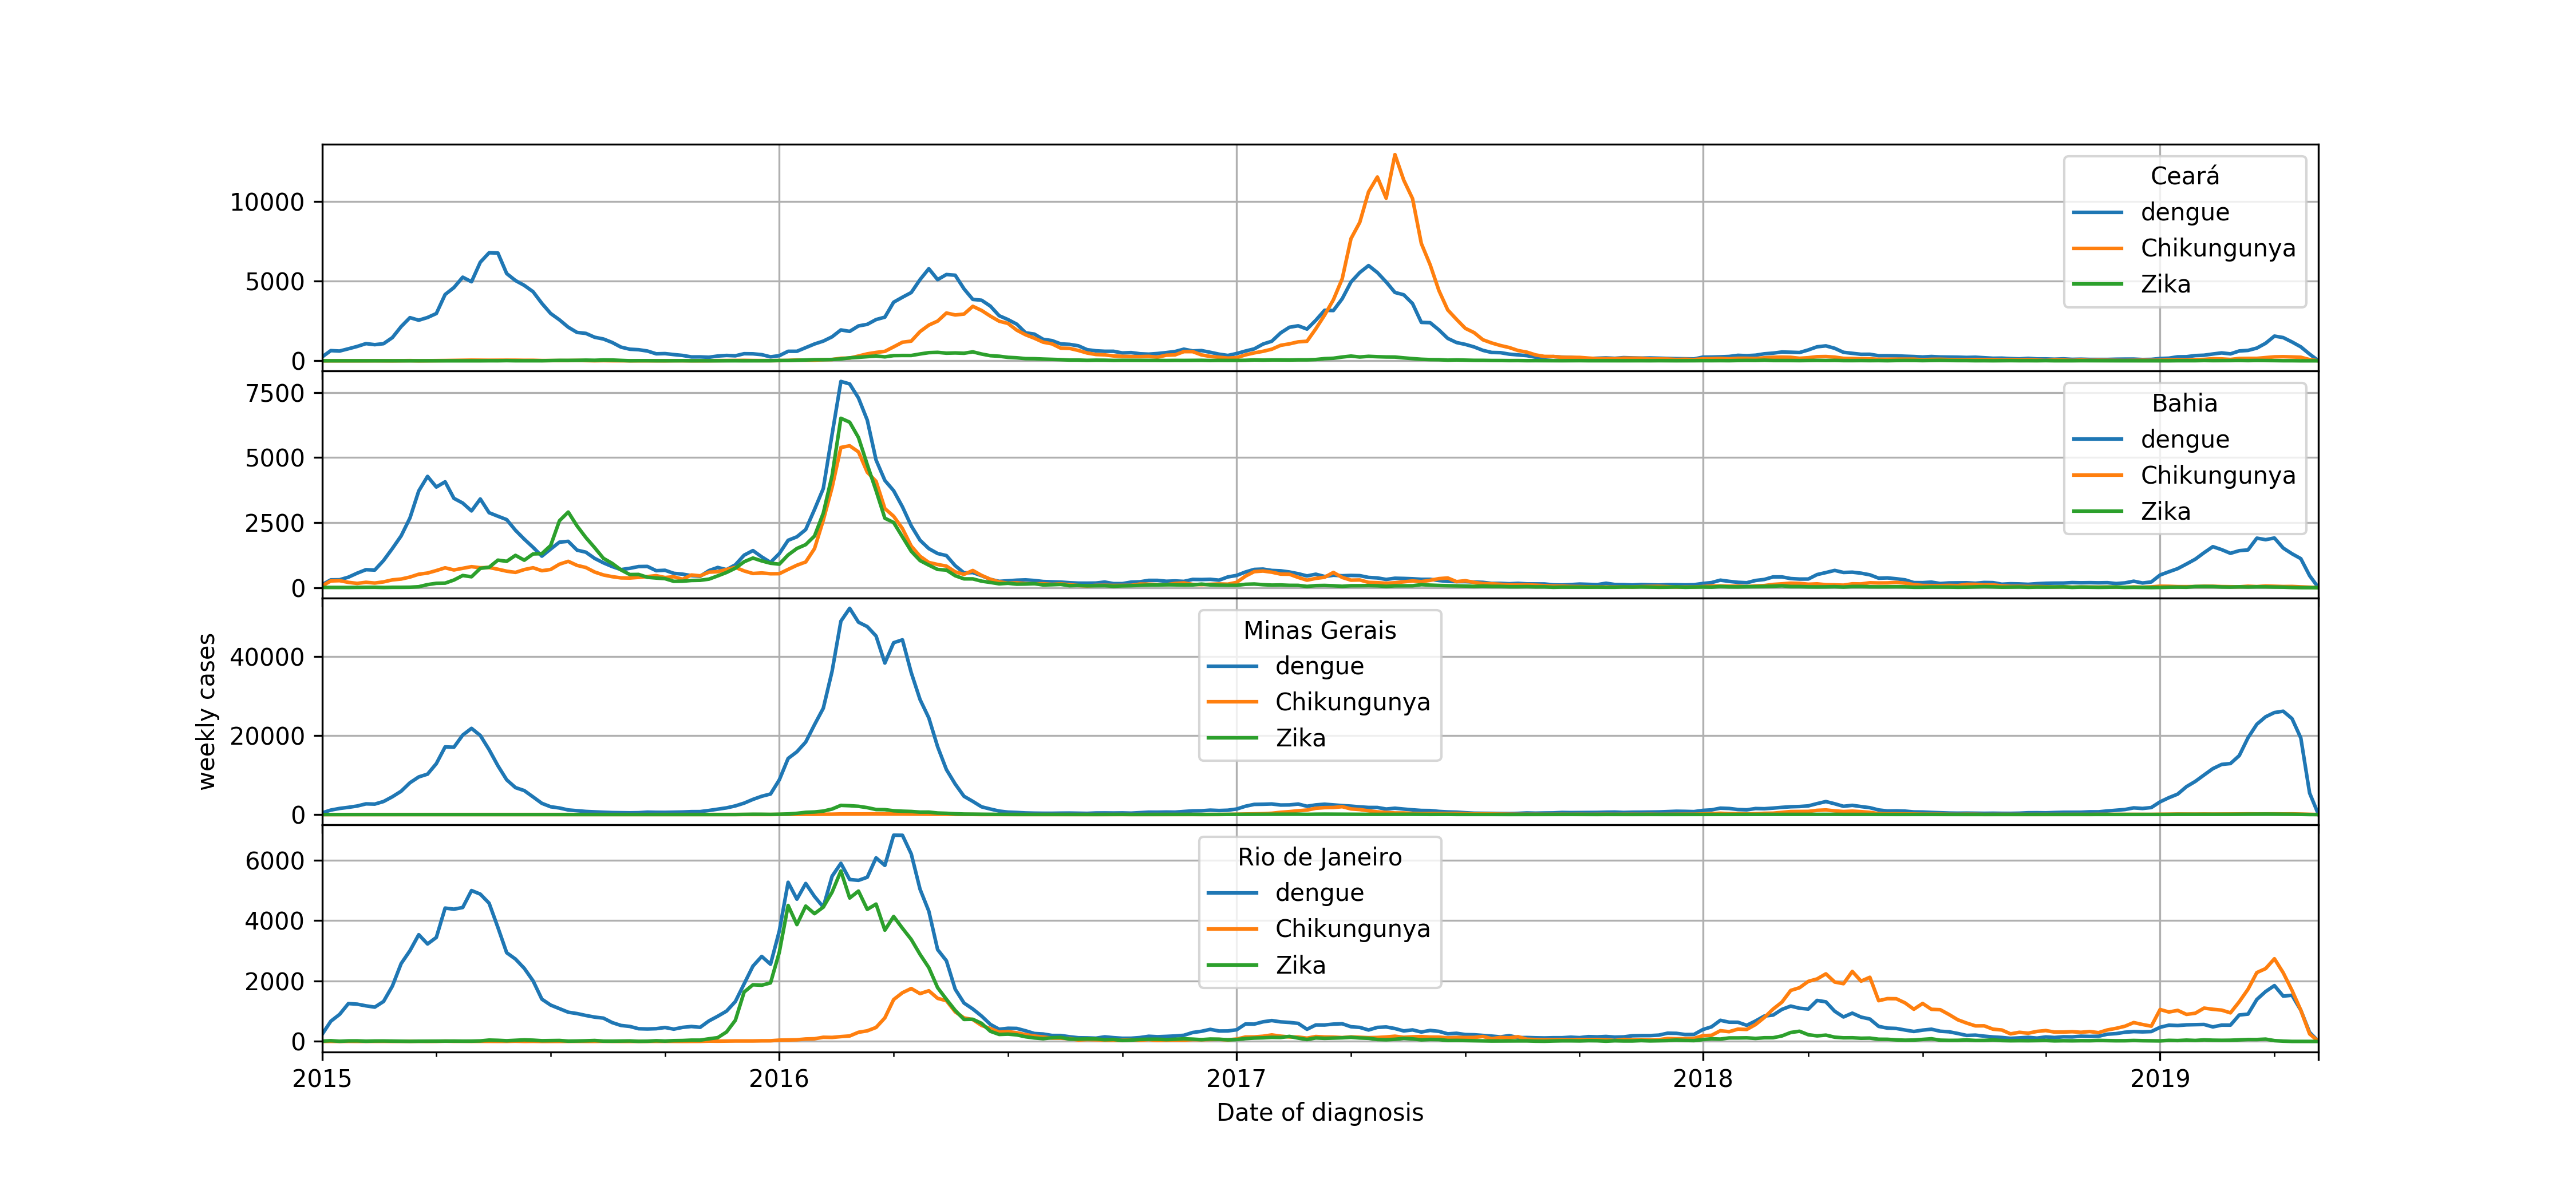
\includegraphics[width=\linewidth]{figures/dcz_series.png}
\captionof{figure}{\textbf{Quality and resolution assessment with NanoJ-SQUIRREL.} \textbf{a)} A super-resolution rendering and acquired widefield image of fixed Alexa647 labelled microtubules. \textbf{b)} Left: SQUIRREL error map highlighting discrepancies between the super-resolution and diffraction-limited images in (a). Right: Magnified insets at indicated positions on error map. \textbf{c)} Left: SQUIRREL resolution map of the super-resolution image in (a). Right: Magnified insets for indicated resolution blocks. Whole image scale bars = 5 \textmu{}m, inset scale bars = 1 \textmu{}m.}
\end{center}%\vspace{1cm}

%----------------------------------------------------------------------------------------
%	NanoJ-VirusMapper: Structural Mapping and Modelling
%----------------------------------------------------------------------------------------
\section*{Conclusion}



\begin{center}\vspace{1cm}
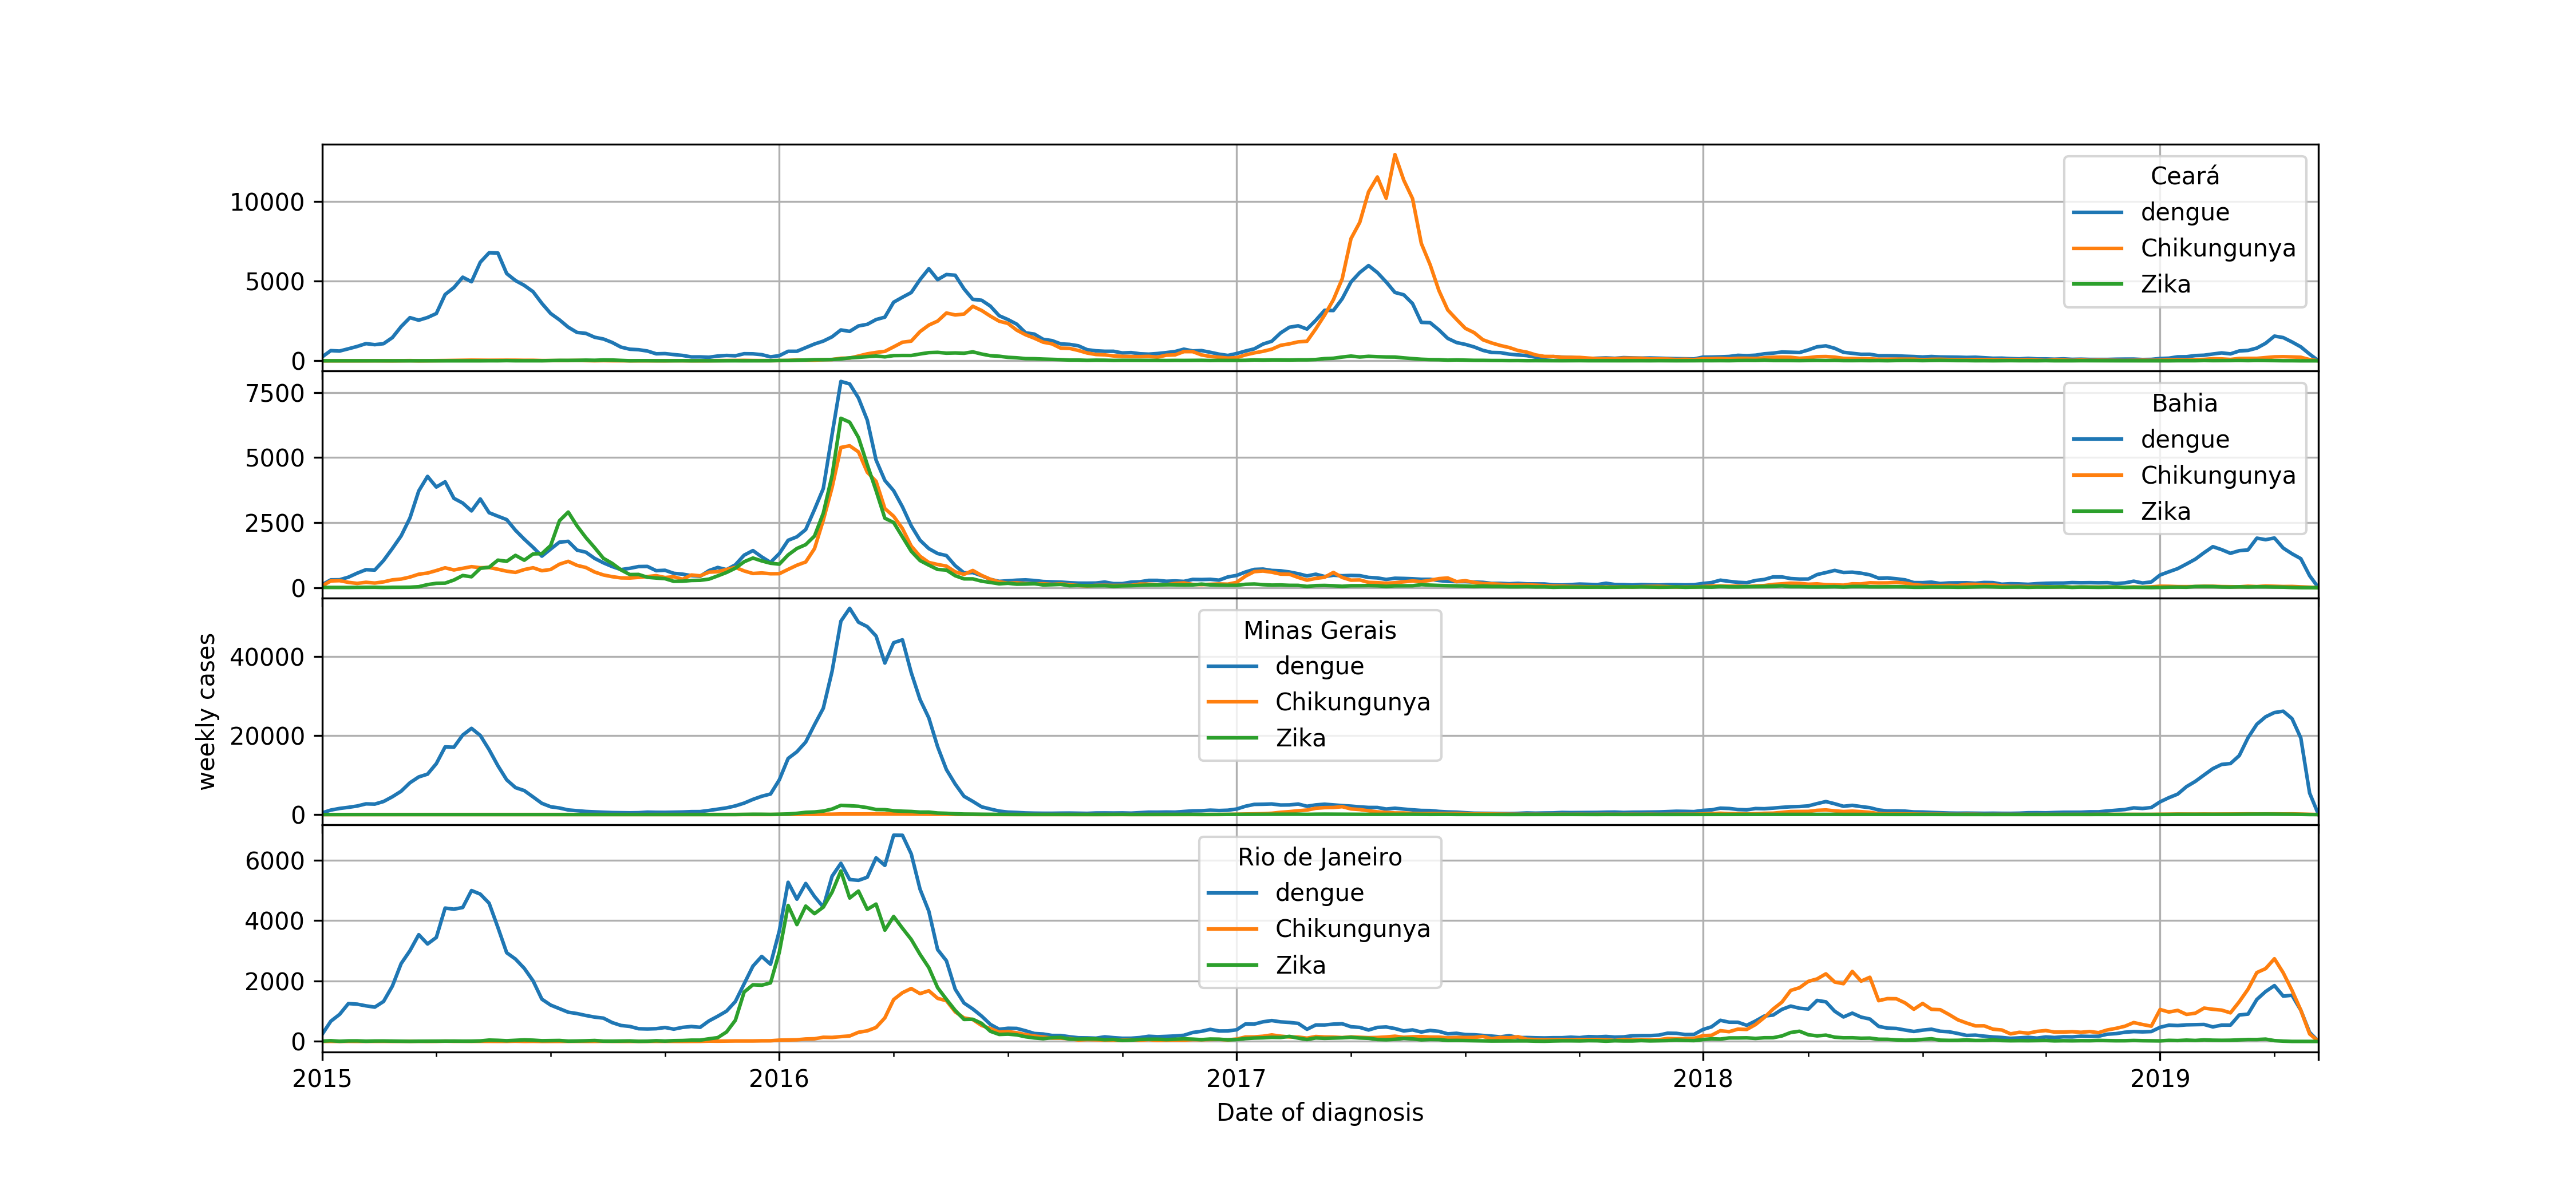
\includegraphics[width=\linewidth]{figures/dcz_series.png}
\captionof{figure}{\textbf{Quantitative SPA-based modelling.} Multicomponent model of the Vaccinia virus by imaging in super-resolution hundreds of fluorescently labelled viruses and modelling their structure through VirusMapper}
\end{center}%\vspace{1cm}

%----------------------------------------------------------------------------------------
%	NanoJ-Fluidics: Sample Liquid Exchange
%----------------------------------------------------------------------------------------



\begin{center}\vspace{1cm}
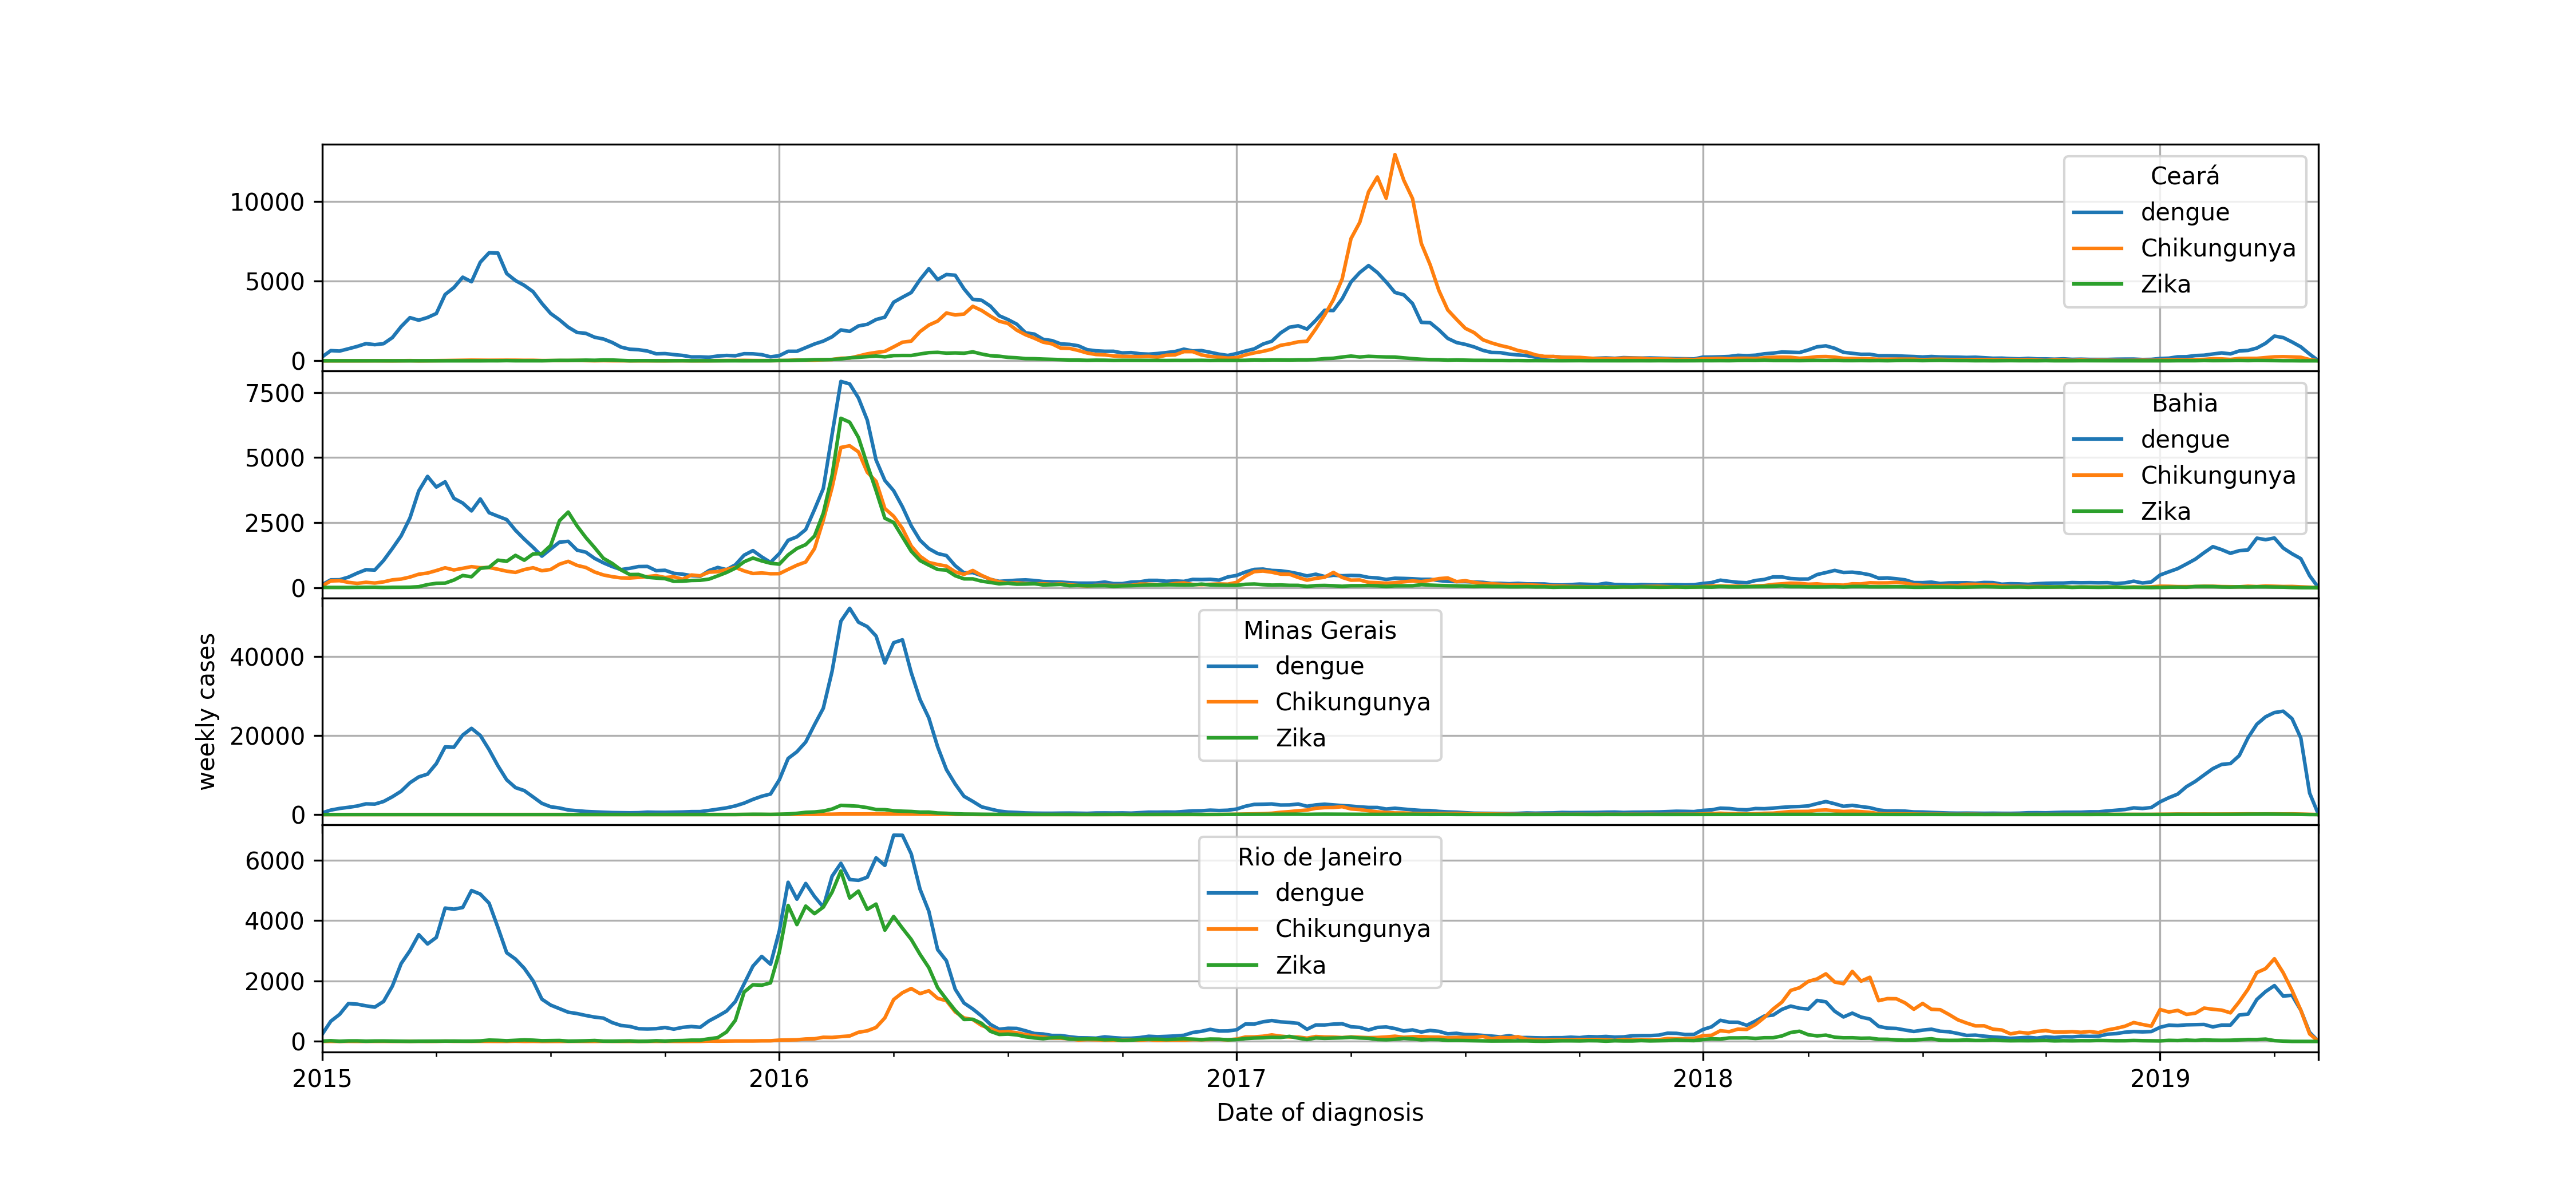
\includegraphics[width=1\linewidth]{figures/dcz_series.png}
\captionof{figure}{\textbf{Schematics of the NanoJ-Fluidics system.} \textbf{a)} 3D side view of a single syringe pump. \textbf{b)} 2D top view of a syringe pump array (representing 4 pumps out of 128 maximum) and a fluid extraction peristaltic pump, both controlled by an Arduino UNO. \textbf{c)} Example of possible workflows}
\end{center}%\vspace{1cm}


% %----------------------------------------------------------------------------------------
% %	CONCLUSIONS
% %----------------------------------------------------------------------------------------

% \section*{Conclusions}
% blabla




%----------------------------------------------------------------------------------------
%	References
%----------------------------------------------------------------------------------------

\small
\nocite{*} % Print all references regardless of whether they were cited in the poster or not
\bibliographystyle{plain} % Plain referencing style
\bibliography{sample} % Use the example bibliography file sample.bib


%----------------------------------------------------------------------------------------
%	Funding
%----------------------------------------------------------------------------------------
\section*{Funded by}
\begin{center}\vspace{0cm}
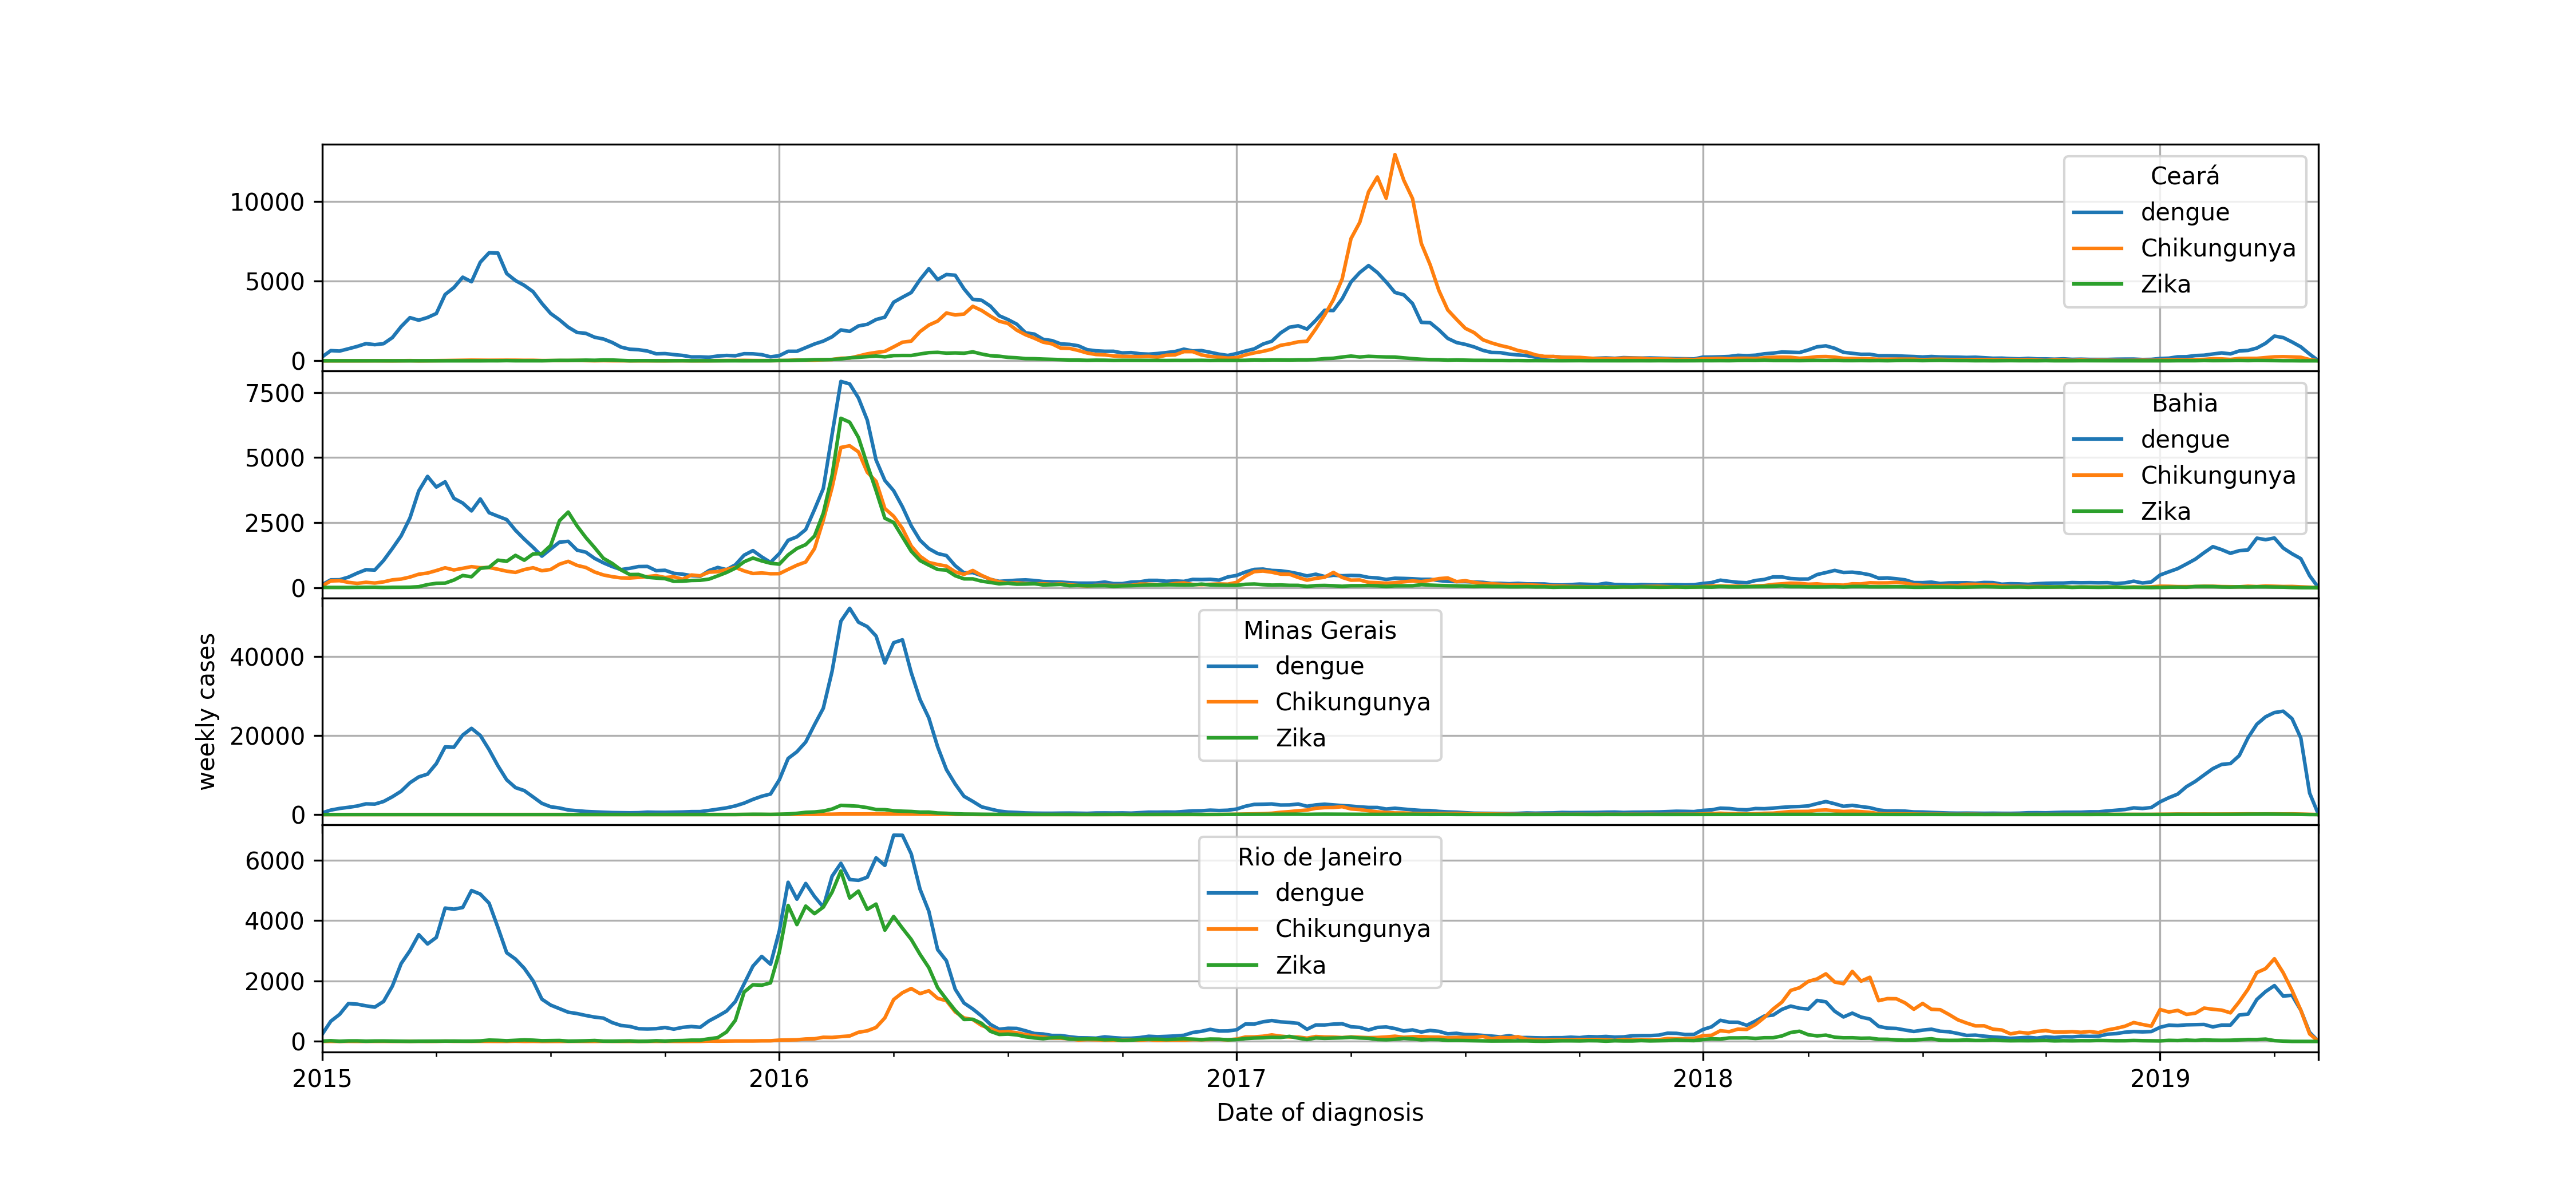
\includegraphics[width=0.95\linewidth]{figures/dcz_series.png}
\end{center}%\vspace{1cm}

%----------------------------------------------------------------------------------------

\end{multicols}
\end{document}
